\documentclass{article}
\usepackage[utf8]{inputenc}
\usepackage{amsmath}
\usepackage{mathtools}
\usepackage{relsize}
\usepackage{graphicx}
\graphicspath{ {./drift/} }
\DeclarePairedDelimiter{\ceil}{\lceil}{\rceil}
\usepackage{geometry}
\usepackage[banglamainfont=Kalpurush, 
            banglattfont=Siyam Rupali
           ]{latexbangla}
        
\begin{document}
\begin{LARGE}
\begin{center}
Motional Electromotive Force
\end{center}
\end{LARGE}

\textbf{ Motional EMF:} Consider a conducting bar of length $ l $ moving through an uniform magnetic field which points into the page, as shown in Figure 1. Particles with charge $ q>0 $ inside experience a magnetic force $ \vec{F_{B}} = q\vec{v}\times \vec{B} $ that tends to push them upward, leaving negative charges on the lower end.
\begin{center}
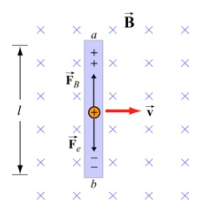
\includegraphics{2018-08-03_152836.png}
\end{center}
The separation of charge gives rise to an electric field $ \vec{E} $ inside the bar, which in turn produces a downward electric force $ \vec{F}_{e} = q\vec{E} $. At equilibrium where the two forces cancel, we have $qvB = qE$, or $E = vB$. Between the two ends of the conductor, there exists a potential difference given by
\[V_{ab} = V_{a}-V_{b} = \varepsilon = El=Blv\]
Since $ \varepsilon $ arises from the motion of the conductor, this potential difference is called the
motional emf.\\
Now suppose the conducting bar moves through a region of uniform magnetic field $ \vec{B} = -B\hat{k} $ (pointing into the page) by sliding along two frictionless conducting rails that are at a distance $ w $ apart and connected together by a resistor with resistance $ R $ , as shown in Figure 2.
\begin{center}
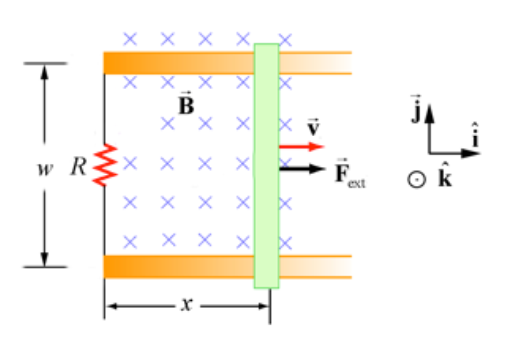
\includegraphics[width=0.5\textwidth]{2018-08-03_152853.png}
\end{center}
Let an external force  $ \vec{F}_{ext} $ be applied so that the conductor moves to the right with a constant velocity $ \vec{v} = v\hat{i}$  . Choose the area element $ \vec{A} = A\hat{k} $ . The magnetic flux through the closed loop formed by the bar and the rails is given by
\[\phi_{B} = \vec{B}\cdot \vec{A} = (-B\hat{k})\cdot (A\hat{k}) = -BA=-Bwx\]
The changing magnetic flux is then
\[ \dfrac{d}{dt}(\phi_{B}) = -\dfrac{d}{dt}(Bwx) = -Bw\dfrac{dx}{dt}=-Bwv\]
where $ \dfrac{dx}{dt} = v $ is the speed of the bar. A charge carrier with charge $ q $ in the moving bar therefore experiences a magnetic force given by
\[F_{B} = q\vec{v}\times\vec{B} = qv\hat{i}\times B(-\hat{k})= qvB\hat{j}\]
We orient the closed path formed by the bar and the rail clockwise so that the unit normal $ \hat{n} = \hat{k} $ (pointing out the page), in order to be consistent with our choice of orientation for the surface integral in our calculation of magnetic flux. The only contribution to the integral is upward along the moving bar. The electromotive force is then

\[\varepsilon = \oint \dfrac{\vec{F}_{B}}{q}\cdot \vec{ds} = \int_{bar} vB\hat{j}\cdot(dy\hat{j}) = wvB \]
where the integral is taken at one instant in time, so the element $ \vec{ds} = dy\hat{j} $ points upward
even though the bar is moving to the right. Comparing Equations, we conclude that

\[\varepsilon = - \dfrac{d\phi_{B}}{dt}\]

The magnetic field is not actually doing the work; the external force that is pulling the bar is doing the work. In order to see why, we first observe that the emf is causing charge carriers to move upward in the bar. The charge carrier has an additional vertical component of velocity

\[\vec{v} = v\hat{i} + u\hat{j}\]

where $ u $ is the $y -$component of the velocity of the charge carriers. Therefore the magnetic force on the charge carrier is given by

\[ \vec{F}_{B}= q\vec{v}\times \vec{B} = q(v\hat{i} + u\hat{j})\times B(-\hat{k}) qvB\hat{j} + quB(-\hat{i})\]

The external force must exactly oppose the $ x- $component of the magnetic force in order
to keep the bar moving at a constant speed,
\[\vec{F}_{ext} = quB\hat{i}\]

If a charge carrier moves from the bottom of the bar to the top of the bar in time $ \triangle t $, then $w = u\triangle t$ . The bar is also moving in the positive $ x- $direction by an amount $\triangle x = v\triangle t = \dfrac{vw}{u} $. The displacement of the moving charge carrier, $ \triangle\vec{s} = (\dfrac{vw}{u})\hat{i} + w\hat{j}$, and the magnetic force are perpendicular because their scalar product is zero,
\[ \vec{F}_{B}\cdot \triangle \vec{s} = (qvB\hat{j} + quB(-\hat{i}))\cdot ((\dfrac{vw}{u})\hat{i} + w\hat{j}) = qvBw - quB(\dfrac{vw}{u}) = 0\]

This is not surprising because magnetic forces do no work. The work done by the external force per charge is equal to the emf,
\[ \int \dfrac{\vec{F}_{ext}}{q}\cdot \vec{ds} = uB\triangle x= uB\dfrac{vw}{u} =vwB = \varepsilon \]
In general, motional emf around a closed conducting loop can be written as

\[ \varepsilon =  \oint(\vec{v}\times \vec{B})\cdot \vec{ds} \]

where $ d\vec{s} $ is a differential length element.
\end{document}